\subsection{Actuators}

    \subsubsection{Thrusters}
        https://www.cubesatshop.com/wp-content/uploads/2017/04/ENP-IFM-Nano-Thruster-Product-Overview.pdf
        https://blog.satsearch.co/2019-07-10-cubesat-thrusters-an-overview-of-in-space-propulsion-products-for-small-satellites

        Parameters:
            Thrust range;
            Nominal thrust: (find a way to model change?)
            Specific impulse (also ranges?)
            Max propellant
            Total impulse
            Power (at nominal thrust?)
            Mass
            Dimensions?
            Hot standby Power
            Time delay to control
            In both directions? 

        % Bang-bang: https://apps.dtic.mil/dtic/tr/fulltext/u2/a291803.pdf
        % /resources/noise_description.pdf

        \begin{figure}[hb]
            \centering
            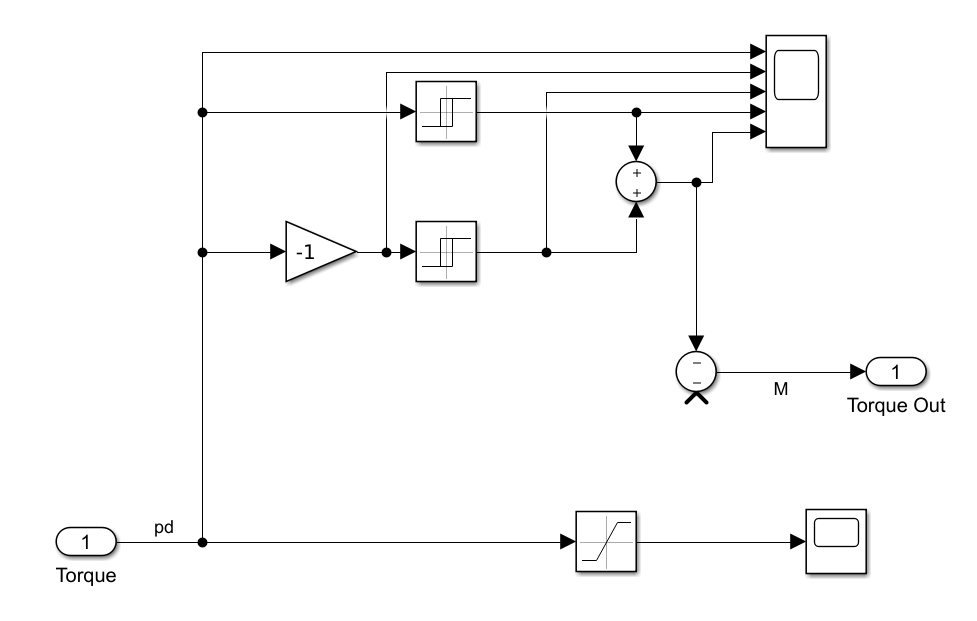
\includegraphics[width=1\textwidth]{2-toolbox/thru_simulink.png}
            \caption{Simulink Thrusters model}
            \label{fig:thru_simulink}
            Thrusters parameters: 
        \end{figure}

    \subsubsection{Reaction Wheels}
        Ideal to real: Bearing Noise, Transport Delay, Saturation, Quantization.
        
        Fast attitude control can be aslo achieved by the use of reaction wheels - mechanisms cosisting of rotating flywheel and proportional electromagnetic torquer, such as DC motor. This allows for very precise attitude maneuvers, with the possiblity to eliminate most disturbance torques. Reaction wheels operate around at a non-zero reference speed and change in their angular velocity imposes corresponding torque on the spacecraft. The disadvantage of this solution is that reaction wheels have fixed operating range and to achieve higher angular velocities for the spacecraft, the wheels have to be desaturatred using another actuators. In cubesats, for example, most commonly this would be solved by the addition of magnetorquers.

        In fast attitude control the motion about each spacecraft body axis can be considered to be decoupled from motion about two other axes. The equations of montion that describe the influence of reaction wheels angular velocity $\dot{q_w}$ on total angular momentum $H$ are as follows:
        
        % \begin{equation}
        \begin{align}
            I_y\dot{q} &= Ni+Q_f+Qdy\\
            \dot{\Theta} &= q\\
            J\dot{q_w} &= -Ni-Q_f\\
            Ri &= e - N(q-q_w)\\
            Q_f &= -c(q-q_w)\\
            H &= I_yq + Jq_w
        \end{align}
        % \end{equation}

        Where $e$, $i$, $R$ are respectively steering voltage, current in DC motor and armature resistance. $N$ is torque per unit current and $c$ is viscous friction coefficient. Said equations were modelled in the toolbox with a following diagram: 
        
        \begin{figure}[hb]
            \centering
            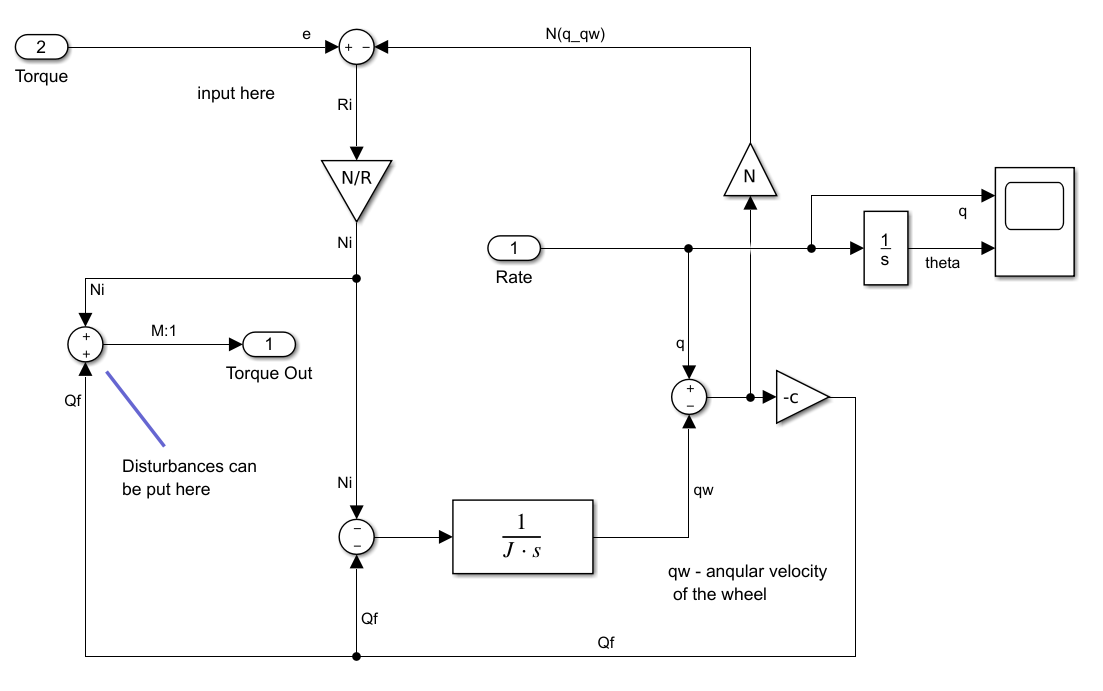
\includegraphics[width=1\textwidth]{2-toolbox/rw_simulink.png}
            \caption{Simulink Reaction Wheels model}
            \label{fig:rw_simulink}
        \end{figure}

        The problem with modeling off-the-shelf reaction wheels is that datasheets rarely provide the value of viscous friction coefficient $c$ in the DC motor. Therefore to model this kind of actuator, \ac{scars} requires the user to only input following data, with $c$ being optional:

        
        \subsubsection{Gimbaled Momentum Wheel}

        %here goes the table


    \subsubsection{Magnetorquers}


    \subsubsection{Deorbitation Sail}


